
\subsection{Double Polarization Experiments}
\label{subsec:poltransfer}



Indeed both the recoil polarization method, and asymmetry measuremnt using polarized target, has been used to measure 
the proton and the neutron form factors. Here we first describe the proton form factor results,  
and next the neutron form factor results. 

\subsubsection{Proton form factor results}

The earliest polarization experiments, measuring polarization of recoil proton \cite{bizot}, and
measuring asymmetry using polarized proton target \cite{powell}, with unpolrized electron beams,
were done to search for the two photon effects.  

The first experiment with polarized electron beam and polarized tartget was done at the Stanford 
Linear Accelerator Center (SLAC) in 1970's \cite{alguard}. 
This experiment measured the beam-target asymmetry $A=\frac{\sigma_{+} -\sigma_{-}}{\sigma_{+} + \sigma_{-}}$
at $Q^2$ = 0.765 GeV$^2$. The experiment concluded that the theoretical and experimental values are in 
good agreement if signs of $G_{Ep}$ and $G_{Mp}$ are the same. 

The first experiment that used the recoil polarization method to measure the proton form factor ratio $G_{Ep}/G_{Mp}$ 
was performed at the MIT-Bates laboratory \cite{milbrathA,barkhuff}. In this experiment the proton 
form factor ratio $G_{Ep}/G_{Mp}$ was measured for a free proton, and for a bound proton in a deuterium 
target at two $Q^2$ = 0.38 and 0.5 GeV$^2$. The success of this experiment elucidated that 
the recoil polarization transfer technique showed great promise for future measurements of $G_{E}$ and 
$G_{M}$ at higher $Q^2$ values for the proton and the neutron. 

Next, using the same method of measuring recoil polarizatrion in $^1H(\vec e,e' \vec p)$ reaction 
the ratio $G_{Ep}/G_{Mp}$  was measured at the MAMI  \cite{pospischil,dietrich} at 
a $Q^2$ of $\approx$0.4 Gev$^2$. The ratio results were in agreement with other polarization 
measurements as well as Rosenbluth measurements. 

In two experiments in Hall A at JLab the proton form factor ratios, $G_{Ep}/G_{Mp}$, were measured for $Q^{2}$ 
from 0.5 to 3.5 GeV$^{2}$ in 1998 and from 4.0 to 5.6 GeV$^2$ in 2000, using the recoil polarization 
method~\cite{jones,gayou:2002,punjabi05A}. 
THe ratios were also measured in 1990's in Hall A \cite{gayou:2001,strauch,hu} at lower $Q^2$ values, as 
calibration measurements for other polarization experiments, and one measurement in Hall C \cite{mac}, using the same method. 

The first JLab experiment, GEp(1), measured the ratio, $G_{Ep}/G_{Mp}$,  
up to $Q^{2}$ of 3.5~GeV$^{2}$~\cite{jones,punjabi05A}. In this experiment protons
and electrons were detected in coincidence in the two high-resolution
spectrometers (HRS) of Hall A \cite{nimhallA}. The polarization of the recoiling 
proton was extracted from the azimuthal asymmetry measurement of the 
re-scattered proton in a graphite analyzer.

In the second JLab experiment, GEp(2), the ratio, $G_{Ep}/G_{Mp}$, was measured at $Q^{2}$ = 4.0, 4.8 and 5.6 GeV$^{2}$ with an overlap 
point at $Q^{2}$ = 3.5 GeV$^{2}$ ~\cite{gayou:2002,puckett:2011}. 
Several changes were made compared to the first experiment to extend the measurement to
higher $Q^2$. First, to increase the coefficient-of-merit (COM) of the focal plane 
polarimeter (FPP), a CH$_{2}$ analyzer was used instead of graphite; hydrogen has 
much higher analyzing power \cite{spinka,dmiller} than carbon \cite{cheung}, and to 
increase the fraction of events with a second scattering in the analyzer the
thickness of the analyzer was increased from 50 cm of graphite to 100~cm of CH$_{2}$.
Second, to achieve complete solid angle matching with the 
HRS detecting the proton, a large frontal area lead-glass calorimeter was used to detect the electrons. 
The solid angle of the calorimeter was 6 times that of the HRS, at the largest $Q^{2}$ of 5.6 GeV$^2$. 

The proton form factor ratio also has been measured in a $\vec {^1H}(\vec e,e'p)$ reaction at a $Q^2$ of 1.51 GeV$^2$ 
by measuring the beam-target asymmetry in an experiment in Hall C at JLab in elastic $ep$ scattering \cite{Jones06}.
This is the highest $Q^2$ at which the $G_{Ep}/G_{Mp}$ ratio has been obtained from a beam-target asymmetry measurement. 
This method ws also used  by the BLAST group at MIT-Bates \cite{crawford}; this experiment measured the ratio at $Q^2$ values 
of 0.2 to 0.6 GeV$^2$ with high precision \cite{crawford}.  


%%%%%%%%%%%%%%%%%% 
\begin{figure}
\begin{center}
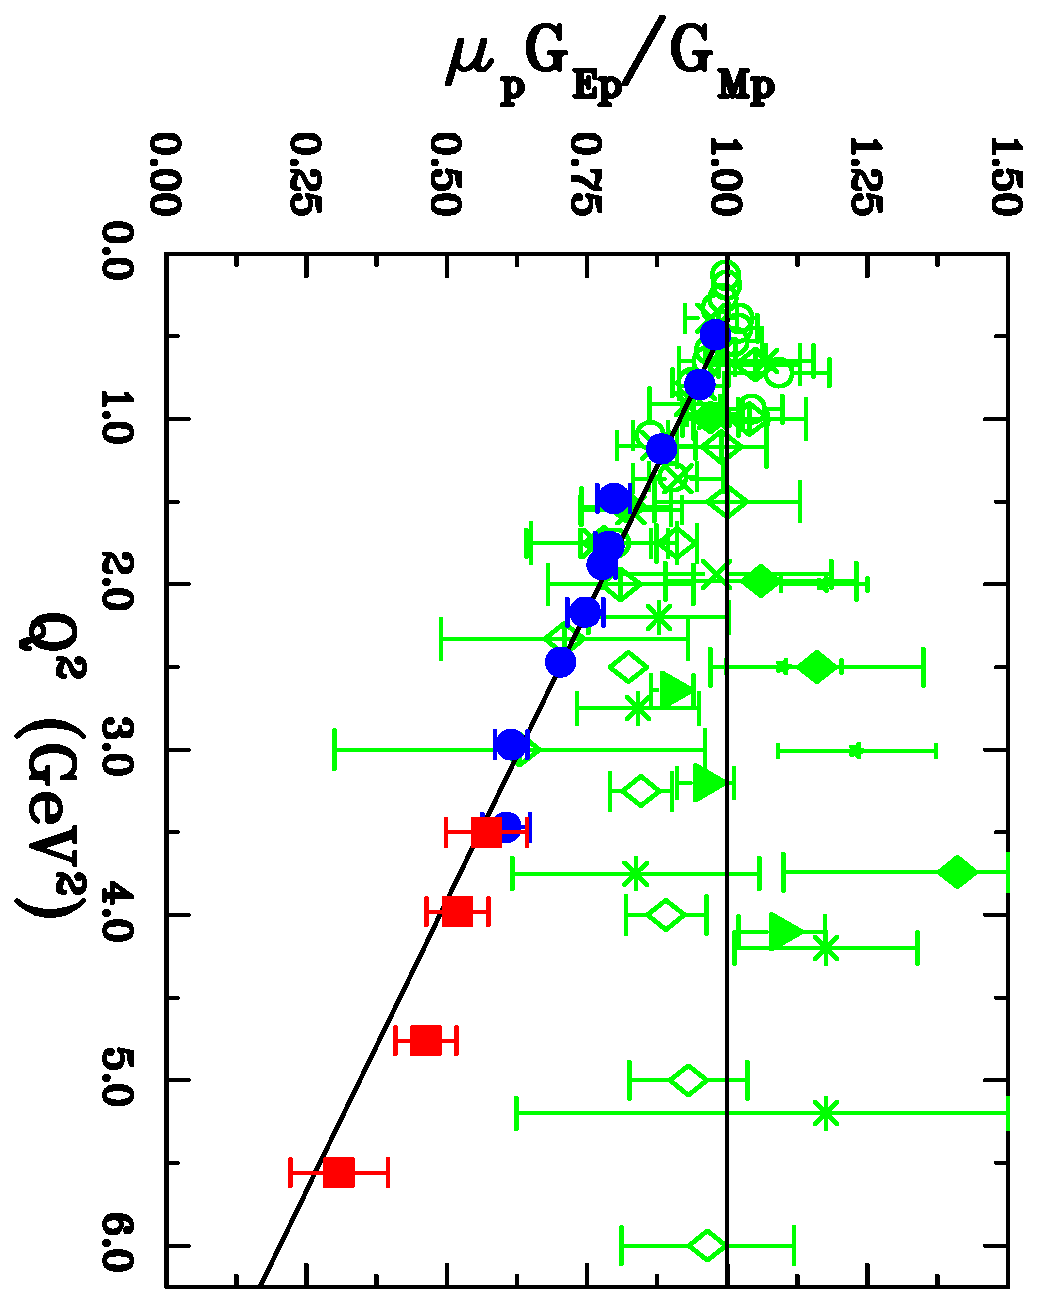
\includegraphics[width=65mm,angle=90]{gepgmp_world_027_bw_p.eps}
\caption{The ratio $\mu_p G_{Ep}/G_{Mp}$ from the two JLab experiments \cite{gayou:2002,punjabi05A} (filled circle and square),
and other polarization experiments, compared to Rosenbluth separation results; JLab Rosenbluth 
results from \cite{christy,qattan05} shown as open and filled triangles, respectively. The cross section data  
in Figs.~\ref{fig:gepgd} and \ref{fig:gmpgd} (open circles).} 
\label{fig:gepgmp_pol_cs}
\end{center}
\end{figure} 
%%%%%%%%%%%%%%%%%%%

The results from the two JLab experiments \cite{jones,punjabi05A,gayou:2002}, are plotted 
in Fig.~\ref{fig:gepgmp_pol_cs} as the ratio $\mu_{p}G_{Ep}/G_{Mp}$ versus $Q^2$, where they are also
compared with Rosenbluth separation data \cite{andivahisA,christy,qattan05,wilsonrr,berger,bartel,price,hanson,litt}.
As can be seen from figure \ref{fig:gepgmp_pol_cs}, for the polarization data the statistical
uncertainty is small; this is unlike the cross section data, 
where we see a large statistical uncertainty at higher $Q^2$ values, underlining
the difficulties in obtaining $G_{Ep}$ by the Rosenbluth separation method, as well as a large scatter 
in results from different experiments. 
The ratio $G_{Ep}/G_{Mp}$ from polarization experiments decreases almost linearly
with $Q^2$, revealing a definite difference between the spatial distributions of charge and magnetization at 
short distances. These results were very surprising at the time (1998-2002), as they appeared to contradict 
the consensus based on Rosenbluth separation results up to 6 GeV$^2$ by Andivahis {\it et al.} \cite{andivahisA} that demonstrated 
that the ratio, $\mu_{p}G_{Ep}/G_{Mp}$, remains close to 1 as illustrated in Fig.~\ref{fig:gepgmp_pol_cs}. 

The results from the two JLab experiments \cite{jones,punjabi05A,gayou:2002} showed 
conclusively for the first time a clear deviation of
the proton FF ratio from unity, starting at $Q^2\simeq 1$~GeV$^2$; older data from \cite{berger,price,bartel,hanson}
showed such a decreasing ratio, but with much larger statistical and systematic uncertainties, as seen in Fig. 
\ref{fig:gepgmp_pol_cs}. 
The most important feature of the JLab data, is the sharp decrease of the ratio
$\mu_p G_{Ep}/G_{Mp}$ from 1 starting at $Q^2$ $\approx$ 1 GeV$^2$ to a value of
$\sim 0.28$ at $Q^2$= 5.6 GeV$^2$, which indicates that $G_{Ep}$ falls 
faster with increasing $Q^2$ than $G_{Mp}$. This was the first definite experimental indication
that the $Q^2$ dependence of $G_{Ep}$ and $G_{Mp}$ is different. 

The two methods, Rosenbluth and polarization,  give definitively 
different results; the difference cannot be bridged by either simple re-normalization 
of the Rosenbluth data \cite{arring03}, or by variation of the polarization data within the 
quoted statistical and systematic uncertainties. This discrepancy has been known
for sometime now, and has been the subject of discussion and investigation. 
A possible explanation is the hard two-photon exchange process, which affects 
both cross section and polarization transfer components at the level of only a few percents; 
however, the contribution of the two-photon process has drastic effect on the  Rosenbluth 
separation results, whereas it modifies the 
ratio obtained with the polarization method by a few percent
only. This will be discussed in detail in \ref{sec:twophoton}.

Following the unexpected results from the GEp(1) and GEp(2) polarization experiments at JLab, a new 
experiment, GEp(3) was approved to extend the Q$^2$-range to 9 GeV$^2$ in Hall C at JLab. 
Two new detectors were built to carry out this experiment; a large solid-angle electromagnetic 
calorimeter and a double FPP. The recoil protons were detected in the 
high momentum spectrometer (HMS) equipped with the new double FPP. The scattered electrons were
detected in a new lead glass calorimeter (BigCal) built for this purpose out of
1744 glass bars, 4x4 cm$^2$ each, giving a total frontal area of 2.6 m$^2$, 
which provided complete kinematical matching to HMS solid angle. 
This experiment was completed in the spring of 2008 and measured the form 
factor ratio at $Q^2$ of 5.2, 6.7 and 8.5 GeV$^2$. The data analysis
was completed in 2010 and the results were published \cite{puckett:2010}. 

\begin{figure}
\begin{center}
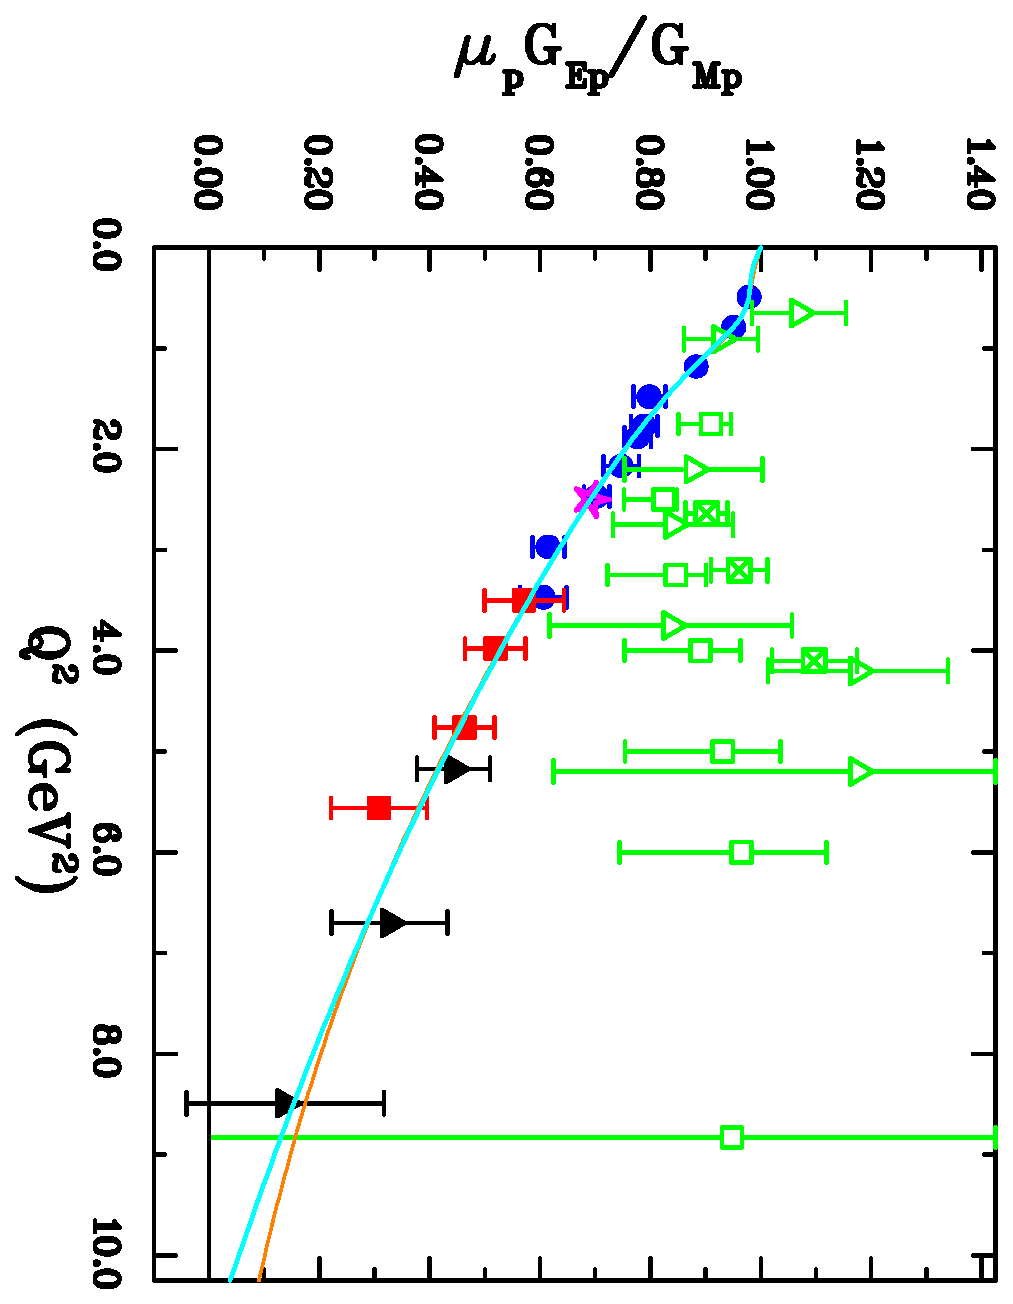
\includegraphics[width=65mm,angle=90]{gepgmp_allpol_allcs_noth_11072014.eps}
\caption{All data for the ratio $G_{Ep}/G_{Mp}$ obtained from the three large $Q^2$ recoil polarization experiments at 
JLab and all other double polarization experiments. The dot-dashed curve is a 4 parameter fit without constrain at $Q^2$=0, the solid line is a 7 parameter 
fit with ratio constrained to 1 at $Q^2$=0; Both fits are of the Kelly type, polynomial over polynomial, with $1/Q^2$ behavior at large $Q^2$.}
\label{fig:gepgmp_all_pol}
\end{center}
\end{figure}

Figure \ref{fig:gepgmp_all_pol} shows the results from three JLab experiments \cite{jones,gayou:2002,punjabi05A,puckett:2010}, as well as results of 
all other double polarization  experiments \cite{milbrathA,gayou:2001,pospischil,dietrich,strauch,hu,mac,Jones06,crawford,paolone:2010}, as the 
ratio $\mu_{p}G_{Ep}/G_{Mp}$ versus $Q^2$. All data show only the statistical uncertainty. As can be seen from figure \ref{fig:gepgmp_all_pol}, data from 
different experiments are in excellent agreement, this is unlike $G_{Ep}$ obtained from cross section data. 

The striking feature of the results of the GEp(3) experiment is a continued, strong and almost linear
decrease of the ratio with increasing Q$^2$, albeit with some indication of a slowdown at the highest Q$^2$. 
The overlap point at $5.2$ GeV$^2$ is in reasonably good agreement with the two 
surrounding points from Gayou {\it et al.} ~\cite{gayou:2001}. The GEp(3) experiment used a completely different 
apparatus in a $Q^2$ range where direct comparison with the Hall A recoil polarization 
results is possible. The comparison provides an important confirmation of the reproducibility 
of the results with the recoil polarization technique using a completely different apparatus.
Additionally, the results of the high-statistics survey of the $\epsilon$-dependence 
of $G_{Ep}/G_{Mp}$ at $Q^2=2.5$ GeV$^2$, from the GEp($2 \gamma$) experiment \cite{Meziane:2010}
shown as magenta star in  
Fig.~\ref{fig:gepgmp_all_pol} is in excellent agreement with the results from GEp(1) experiment in Hall A~\cite{punjabi05A} 
at $Q^2=2.47$ GeV$^2$.

Fig. \ref{fig:q2f2f1} shows the ratio of the 
Pauli and Dirac form factors, $F_2$ and $F_1$, multiplied by $Q^2$, which can be  obtained directly
from the ratio $G_{Ep}/G_{Mp}$, without requiring any additional information; this is the 
second interesting result of this experiment: the ratio $Q^2{F_2/F_1}$ does not show an obvious tendency 
to become constant, as the original perturbative QCD prediction of Brodsky 
et al~\cite{brodsky} implied.  




